\section{Query evaluation}

In this section, we explain how to evaluate queries with the given data set. For this query evaluation we can use a distributed event stream processing system with the process graph as shown in Figure \ref{twonode_graph} for both queries.

\begin{figure}[!t]
        \centering
        \includegraphics[width=3.0in]{twonode_graph.png}
        \caption{Two node process graph to evaluate queries}
        \label{twonode_graph}
\end{figure}

\textit{EventEmitter} reads the data file and generates events. For real implementation, each query has its own \textit{EventEmitter} which reads each line of the data file and generates an event with relevant information. \textit{QueryEvaluator} evaluates the query against the received event and generates top ten value changed event.  In general we can evaluate queries sequentially and parallel. In a sequential execution, all events goes to one \textit{QueryEvaluator} instance and in parallel execution, event stream is partitioned using the key field and evaluate simultaneously with different \textit{QueryEvaluator} instances.

\subsection{Sequential evaluation}

We can sequentially execute events either in a single Java Virtual Machine (JVM) or different JVMs (either in one machine or different machines) using TCP sockets to communicate between process instances. Figure \ref{sequential} shows such possible executions. 

\begin{figure}[!t]
        \centering
        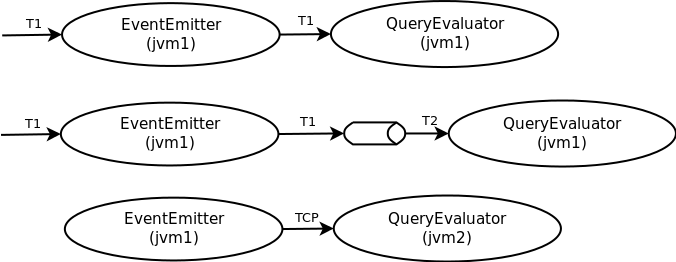
\includegraphics[width=3.0in]{sequential.png}
        \caption{Different types of sequential execution}
        \label{sequential}
\end{figure}

First both processors can be executed in same JVM with same thread. In that case both processes executes sequentially. We can make two processes parallel by executing them with two threads and communicate using a queue in same JVM or communicate using a TCP connection for different JVMs. In all these cases \textit{QueryEvaluator} processes messages sequentially and becomes the bottleneck. Next we show how to parallel \textit{QueryEvaluator} process. 


